% ============================================================
% Master file for the appendices.
% In the main document, replace the old
%     \appendix
%     \include{Appendix A}
%     \include{Addenda}
% (or whatever the template uses) with:
%     \appendix
%     \input{appendices/appendices}
%
% Order follows the first reference to each appendix in the body of the
% report. Appendix A is fixed by the template (GA summary).
% ============================================================
\chapter{Graduate Attributes}
\label{appendix:GA}

The table below summarises how the graduate attributes (GAs) associated with this course have been met, and where in the report the evidence can be found.

\setlength{\LTcapwidth}{\linewidth}
\begin{longtable}{|>{\centering\arraybackslash}p{0.05\linewidth}
		|>{\raggedright\arraybackslash}p{0.17\linewidth}
		|p{0.66\linewidth}||}
	\caption{Graduate attributes and where they are addressed in this report}
	\label{tab:GAs}\\
	\hline
	\textbf{GA} & \textbf{Requirement} & \textbf{Justification and section in the report} \\ [0.5ex]
	\hline\hline
	\endfirsthead
	
	\multicolumn{3}{l}{\small\itshape \tablename~\thetable{} (continued)}\\
	\hline
	\textbf{GA} & \textbf{Requirement} & \textbf{Justification and section in the report} \\ [0.5ex]
	\hline\hline
	\endhead
	
	\hline
	\multicolumn{3}{r}{\small\itshape Continued on next page}\\
	\endfoot
	
	\hline
	\endlastfoot
	
	1 & Problem-solving & My project concerns the field of LiDAR for wind-speed measurement. Specifically, my project deals
	with the problem of designing a prototype benchtop-scale version of a Doppler wind LiDAR system. I
	consulted various sources of literature in order to first understand what the key use-cases and goals of
	Doppler wind LiDAR systems are (mostly with respect to wind-turbines, and the use of such systems to
	control the turbines optimally). Thereafter, with the end-use in mind, I reviewed sources which discuss
	common types/classes of such systems (\autoref{sec:litReview}), and identified a system type which would be suitable for this
	project, given the time-frame and budget -- this type being coherent detection Doppler LiDAR (\autoref{sec:design-sysArch}).
	After identifying this suitable class of system, I reviewed the various design considerations of such a
	system in the available literature (\autoref{sec:litReview}). This included mathematical and physical descriptions of how the
	system operates, with respect to signal theory, optics, electronics, and relevant physics phenomena
	(including Rayleigh and Mie scattering, coherent detection methodology, balanced detection, and
	laser source physics). From this, I synthesised a list of parts which would be suitable for use in the project, and used the relevant mathematics to validate these choices in terms of the final
	requirements (\autoref{sec:design-ComponentChoices}, \autoref{sec:design-sysReqs}).
	\\
	\hline
	4 & Investigations, experiments and data analysis & I conducted a thorough investigation into the various types of Doppler wind LiDAR systems which are
	used in industry and scientific research. After doing so, I conducted more specific research into
	coherent detection Doppler LiDAR systems, and the physics, signal processing and optics which
	underpin these systems (\autoref{sec:litReview}, \autoref{sec:design-ComponentChoices}). From this, I was able to recommend to my supervisor a course of action for
	the class of system to be designed, and substantiate this choice through the research done.
	I formulated various experiments to conduct on the system once it
	was built, which validate the signal theory, mathematics and electronics principles
	concerned, and validate the system's workings (\autoref{sec:noiseAnalysis}, \autoref{sec:functionalTesting}). The primary consideration in these experiments is a thorough noise analysis (\autoref{sec:noiseAnalysis}), which
	serves to quantify the sensitivity of the system. Furthermore, the effects of various design decisions on the
	performance (e.g.\ source laser linewidth and power, or the use of balanced detection over single-ended detection) are analysed in these experiments, and optimal requirements for such systems
	are thus experimentally shown and discussed, and suitable recommendations for upgrades are made. \\
	\hline
	5 & Use of engineering tools & Engineering mathematics was used in the system's design in order to determine the optimal components to use (e.g.\ the fibre-optic splitter ratio in \autoref{sec:design-ComponentChoices}). Reasoning based on the reviewed literature was applied to predict performance outcomes and to determine how the system should be tested (e.g.\ the prediction that the system will require seeded air for wind-speed measurement due to the lack of optical power amplification, \autoref{sec:design-ComponentChoices}). Once the system was built, an oscilloscope was used in conjunction with Python scripts to acquire data from the system (setup described in \autoref{sec:design-DataAcquisition}, used in \autoref{sec:noiseAnalysis} and \autoref{sec:functionalTesting}). The data was also post-processed using Python scripts so as to gain useful information from it, and to generate plots and tables which show the obtained data in a readable manner. \\
	\hline
	6 & Professional and technical communication (long report) & I have attended scheduled meetings (and scheduled further follow-up meetings) with my supervisor in
	order to discuss the route which the project should take, as well as budget and technological
	considerations. I have also consulted with Maysam Soltanian to obtain suitable sources for components
	which are required for the project.
	
	This written project report serves to communicate the technical details of the system's development and testing to an engineering audience. The abstract and conclusion of this report serve to communicate basic ideas (e.g.\ the need for system upgrades in order to perform wind-speed measurements in clean air) to a non-engineering or management audience. \\
	\hline
	8 & Individual work & I have maintained goals and suggested timeframes for my work on the project. While meetings
	with my supervisor and Maysam helped guide the sourcing and budget constraints for the project
	components, all of the specific components were selected by me, and suitable sourcing suggestions
	were made to Maysam. While the supervisor provided the overarching topic of Doppler wind LiDAR, I
	used my own research into the area to select an appropriate subclass of LiDAR system to build for the
	project, synthesising the constraints of the project and the desired requirements. All experimental work was synthesised individually. Appendix \ref{appendix:AIUse} shows a knowledge of professional ethics and norms in its declaration of how and where artificial intelligence was used in this project. \\
	\hline
	9 & Independent learning ability & I have independently learnt concepts in photonics (laser source characteristics), atmospheric sciences
	(Rayleigh and Mie scattering) and signal theory (coherent detection and balanced detection), in order
	to understand and synthesise the design of a Doppler wind LiDAR system.
	
	The initial problem was ill-defined and the decision to take the route of designing a benchtop-scale
	Doppler wind LiDAR system was not immediately obvious. It was only after learning more about the
	field and evaluating areas of research in it that this decision was made, after reaching out to my
	supervisor to consult on this. Throughout the project I have had to manage the scope of the project to
	suit my abilities and constraints, given that the field of research contains many complexities which are
	beyond an undergraduate skill-level and time-frame. This therefore shows my ability to synthesise
	meaningful objectives, knowledge and outcomes from an ill-posed problem. \\ [1ex]
\end{longtable}
   % A  GA summary (template-mandated)
\chapter{Linewidth, PIIN and Doppler Peak Broadening}
\label{appendix:PIIN}
% Referenced from: Sec 2.5 (noise sources), Sec 3.4.1 (Linewidth),
% Table 3.1 (monostatic row -- change its \autoref{sec:lit-linewidth} to
% \autoref{appendix:PIIN}), Sec 4.3.1, Sec 4.3.3 (fix the "Appendix ??" there
% to \autoref{appendix:PIIN}), Sec 4.3.4.
In order to understand the linewidth property of a laser source, it is important to first have an understanding of the concept of phase noise in a laser:

    An ideal laser emits an electromagnetic wave $E(t) = E_0cos(2\pi f_0t + \phi)$ with $\phi$ a constant. A real laser emits $E(t)=E_0cos(2\pi f_0t + \phi(t))$ where $\phi(t)$ drifts unpredictably. This drift is called phase noise. Thus, when considering the frequency spectrum of the emitted laser beam over a long time period, it takes a Lorentzian shape centred around the nominal frequency of the laser (whereas an ideal laser would present simply as a delta spike at the nominal frequency). The laser linewidth, $\Delta f$, is then defined as the -3dB bandwidth of this Lorentzian spectrum, as illustrated in \autoref{fig:lorentzian} below:

    \begin{figure}[H]
    \centering
    \begin{tikzpicture}
    \begin{axis}[
        width=0.68\textwidth, height=5.5cm,
        xlabel={Frequency},
        ylabel={Normalised PSD},
        domain=-3:3, samples=400,
        xmin=-3.2, xmax=3.2, ymin=0, ymax=1.2,
        axis lines=left,
        xtick={-2,0,2},
        xticklabels={$f_0-2\Delta f$, $f_0$, $f_0+2\Delta f$},
        clip=false,
    ]
    \addplot[thick, black] {1/(1+(2*x)^2)};

    % half-maximum level
    \addplot[dashed, gray] coordinates {(-3.2,0.5) (3.2,0.5)};
    \node[left, gray, font=\footnotesize] at (axis cs:-2.2,0.6) {$-3$\,dB};

    % centre line
    \draw[dotted, gray] (axis cs:0,0) -- (axis cs:0,1);

    % FWHM arrow
    \draw[<->, thick] (axis cs:-0.5,0.5) -- (axis cs:0.5,0.5);
    \node[above, font=\small] at (axis cs:0,0.52) {$\Delta f$};
    \end{axis}
    \end{tikzpicture}
    \caption{Lorentzian frequency spectrum of a laser diode.}
    \label{fig:lorentzian}
    \end{figure}

    Asssociated with the linewidth is a quantity termed coherence length. The coherence length of the emitted beam, $L_c$, is given by \cite{bennett_doppler_2003}:

    \begin{equation}
        L_c = \frac{c}{2\pi\Delta f}
        \label{eqn:coherenceLength}
    \end{equation}

    Where $\Delta f$ is the linewidth of the source laser, and $c$ is the speed of light. The coherence length is of relevance when considering linewidth effects.

    The non-ideal linewidth property of a laser source gives rise to two primary effects in a DWL system's measurements - namely phase-induced intensity noise (PIIN), and the broadened Doppler peak:

    As noted by Cariou et al. \cite{cariou2006laser}, Jiang et al. \cite{jiang_performance_2019}, and Harris et al. \cite{harris_role_1998}, reflections of the outgoing beam - caused by optics and the fibre optic transmit path - travel back in the system and are interfered with the reference beam (LO) before detection (in the same way as the actual backscattered signal of interest is). Because the reflection and LO derive
    from the same source, the mixing product is a strong, unwanted tone at baseband (homodyne)
    or at the intermediate frequency (heterodyne), carrying the phase noise
    accumulated over the path-length mismatch $\Delta L$ between the reflection and the LO. Harris et
    al. \cite{harris_role_1998} show that the form of this residual noise is set by how large
    $\Delta L$ is relative to the coherence length ($L_c$) of the laser source.

    For $\Delta L \gg L_c$ the two
    phases are highly uncorrelated because the difference in path (and therefore time) taken has allowed the phase of the two to "wander" significantly - and thus the tone broadens into a Lorentzian of width
    $2\Delta f$. This case is illustrated in \autoref{fig:commonmode} below, where it can be seen that this unwanted Lorentzian peak can serve to swamp out the desired Doppler peak to be measured - this is especially impactful for low wind-speeds, where the Doppler peak will be closer to the unwanted common-mode Lorentzian peak, and will be hidden more by it.

    \begin{figure}[H]
    \centering
    \begin{tikzpicture}
    \begin{axis}[
        width=0.68\textwidth, height=5.5cm,
        xlabel={Frequency},
        ylabel={PSD},
        domain=-1.5:5, samples=500,
        xmin=-1.5, xmax=5, ymin=0, ymax=1.25,
        axis lines=left,
        xtick={0,2.5},
        xticklabels={$f_0$, $f_0+f_d$},
        ytick=\empty,
        clip=false,
    ]
    % common mode + Doppler signal
    \addplot[thick, black] {1/(1+(3*x)^2) + 0.18/(1+(8*(x-2.5))^2)};

    % centre lines
    \draw[dotted, gray] (axis cs:0,0) -- (axis cs:0,1);
    \draw[dotted, gray] (axis cs:2.5,0) -- (axis cs:2.5,0.2);

    % peak labels
    \node[right, font=\small] at (axis cs:0.3,1.05) {Common mode};
    \node[right, font=\small] at (axis cs:2.7,0.3) {Doppler signal};
    \end{axis}
    \end{tikzpicture}
    \caption{Spectrum of a monostatic CW coherent lidar, showing the Doppler
    signal superimposed on the skirt of the common-mode peak (adapted from \cite{cariou2006laser}).}
    \label{fig:commonmode}
    \end{figure}

    For $\Delta L \ll L_c$, the case where the mismatch between LO and reflection paths is smaller, the reflected signal and the LO will be more correlated in phase.
    Thus, the residual instead appears as a flat excess noise floor across the
    frequency band, of level proportional to $\Delta f\,\Delta L^{2}$
    \cite{harris_role_1998}. This excess noise is termed excess LO noise,
    interferometric noise or phase-induced intensity noise (PIIN), depending on author
    \cite{harris_role_1998,abari_all-fiber_2014,jiang_performance_2019}. For the remainder of this paper, this excess noise will be termed PIIN. PIIN has
    been measured at 5 - 30dB above shot noise in a diode-laser
    lidar \cite{harris_role_1998} and well above shot noise in a fibre-laser
    system \cite{jiang_performance_2019}. Thus, PIIN is a significant noise source which can cause the system to operate far from the ideal shot-noise limit discussed in \autoref{sec:lit-noiseSources}. It is thus clear that to reduce PIIN, a laser with as small a linewidth as possible should be selected, and the path length mismatch, $\Delta L$ between LO and reflection paths should be minimised.

    Another consideration arising due to non-ideal laser linewidth is the broadening of the measurable Doppler peak. This is particularly notable for longer ranges.

    If the coherence length from \autoref{eqn:coherenceLength} is long relative to the emitted signal's path length, the broadening of the Doppler peak due to the laser's linewidth may be neglected, and it will instead be other factors (such as turbulence in the air, and speckle) which dominate and cause a broader measurable peak \cite{bennett_doppler_2003}. This is because the total round-trip time of the beam is shorter, thus ensuring that the phase of the beam has not had "time" to shift significantly in between transmission, and later reception and mixing with the local oscillator. Thus, the received backscatter signal and the LO phase will be more coherent and will result in a sharper peak after mixing.

    Conversely, if the coherence length is short relative to the signal path length (i.e. for targets at greater ranges), the Doppler peak will be spread over $2\times\Delta f$, meaning that the measurement resolution and the ability to resolve turbulence in the air will be reduced \cite{bennett_doppler_2003}.

    From the two effects described above, it can clearly be seen that a narrow linewidth laser source is highly beneficial for DWL systems, in order to achieve the best-case shot-noise limited operation, and to achieve a narrow, measurable Doppler peak.
        % B  first ref: Sec 2.5
\chapter{Balanced Detection}
\label{appendix:RIN}
% Referenced from: Sec 2.6, Table 3.1 (balanced-detection row), Sec 5.1.3 and
% Sec 5.2.3 (via \autoref{eq:beat_power}).
As discussed  in \autoref{sec:lit-noiseSources}, the best-case performance of a DWL system is for it to operate in a shot-noise limited regime - thus, all other sources of noise should be reduced to below the shot-noise level. In coherent detection LiDAR architectures, the use of a balanced detector setup has become common for this purpose, as it assists in reducing a laser source's relative-intensity noise (RIN) below the shot-noise level, in a manner which single-ended detection does not.

A single-ended detection system simply uses a 2:1 (2 inputs, one output) fiber optic coupler to mix the LO reference signal with the backscatter signal, and uses a single photodetector to convert this light signal into a measurable current. It can be seen that this detection method retains the DC terms $P_{LO}$, $P_{RS}$. Any RIN from the laser source is present in the output, as these intensity fluctuations are contained in these two power terms. Thus, the measurable Doppler peak will be smaller with respect to the noise floor.

Contrastingly, balanced detection setup makes use of a 2:2 fibre optic coupler which also optically mixes the LO reference signal with the received backscatter signal (as discussed in \autoref{sec:lit-coherentDetection}). However, the 2:2 coupler has two outputs, thus giving two output signals which can be termed $E_1$ and $E_2$ \cite{kikuchi_fundamentals_2016}:

\begin{equation}
	E_1 = \frac{1}{\sqrt2}(E_{RS} + E_{LO}), \space
	E_2 = \frac{1}{\sqrt{2}}(E_{RS} - E_{LO})
\end{equation}
Where $E_{RS}$ and $E_{LO}$ are the complex electromagnetic fields of the returned backscatter signal and the local oscillator respectively.

Thereafter, the two signals enter the balanced detector, which consists of two matched photodiodes and a transimpedance amplifier to convert their currents into a measurable voltage. The photodiodes respond with currents $I_1$ and $I_2$ respectively, proportional to the intensity of the electromagnetic field incident on it ($|E_{1}|^2$ and $|E_2|^2$ respectively), as was also discussed in \autoref{sec:lit-coherentDetection}. Due to the internal setup of the transimpedance amplifier and the photodiodes in the balanced detector, the output current is then given by \cite{kikuchi_fundamentals_2016}:

\begin{equation}
	I_{det} \propto I_1 - I_2 \propto |E_1|^2 - |E_2|^2 \newline
	\propto 2\sqrt{P_{LO}P_{RS}} cos(2\pi\Delta f t)
\end{equation}

Comparing this to \autoref{eqn:beatSignal}, it can be seen that the DC terms $P_{LO}$ and $P_{RS}$ are no longer present due to them being common-mode in both $I_1$ and $I_2$ and thus being canceled by the subtraction. This therefore lowers the noise floor, as the RIN contained in these terms is also eliminated.

Writing in the photodiode responsivity $R$ and the transimpedance gain $G$ of
the balanced detector, the output voltage of the detector is
\begin{equation}
	V(t) = G\,(I_1 - I_2) = 2GR\sqrt{P_{LO}P_{RS}}\,\cos(2\pi\Delta f\,t),
	\label{eq:beat_voltage}
\end{equation}
where $P_{LO}$ and $P_{RS}$ are the total LO and received powers entering the
coupler.

It must also be noted that since the mean of $\cos^2$ is $\tfrac{1}{2}$, the mean-square voltage of the beat signal is
\begin{equation}
	\langle V^2 \rangle = 2G^2R^2P_{LO}P_{RS}.
	\label{eq:beat_power}
\end{equation}
Thus, by Parseval's theorem, $\langle V^2 \rangle$ equals the PSD integrated across
the Doppler peak, so a measured excess power can allow one to estimate the received signal power:
$P_{RS} = \langle V^2 \rangle / (2G^2R^2P_{LO})$.


\autoref{fig:balanceddetector} depicts the balanced detection process graphically:
\begin{figure}[H]
	\centering
	\begin{tikzpicture}[font=\small, line width=0.7pt]

		% ---- inputs ----
		\draw[->] (0.3,2.25) -- (2.2,2.25);
		\node[above] at (1.25,2.25) {$E_{LO}$ (LO)};
		\draw[->] (0.3,0.75) -- (2.2,0.75);
		\node[below, align=center] at (1.25,0.75) {$E_{RS}$\\(backscatter)};

		% ---- coupler ----
		\draw[rounded corners=2pt] (2.2,0.25) rectangle (4.0,2.75);
		\node[align=center] at (3.1,1.5) {50:50\\coupler};

		% ---- coupler outputs ----
		\draw[->] (4.0,2.25) -- (9.0,2.25);
		\node[above] at (6.5,2.25) {$E_1 = \tfrac{1}{\sqrt{2}}(E_{RS} + E_{LO})$};
		\draw[->] (4.0,0.75) -- (9.0,0.75);
		\node[below] at (6.5,0.75) {$E_2 = \tfrac{1}{\sqrt{2}}(E_{RS} - E_{LO})$};

		% ---- balanced detector ----
		\draw[rounded corners=2pt] (9.0,-0.25) rectangle (12.0,3.25);
		\node[above] at (10.5,3.25) {Balanced detector};
		\draw[rounded corners=1pt] (9.3,1.85) rectangle (10.5,2.65);
		\node at (9.9,2.25) {PD$_1$};
		\draw[rounded corners=1pt] (9.3,0.35) rectangle (10.5,1.15);
		\node at (9.9,0.75) {PD$_2$};

		% ---- difference ----
		\draw (10.5,2.25) -- (11.0,2.25) -- (11.0,0.75) -- (10.5,0.75);
		\node[above, font=\footnotesize] at (10.75,2.25) {$I_1$};
		\node[below, font=\footnotesize] at (10.75,0.75) {$I_2$};
		\fill (11.0,1.5) circle (1.5pt);
		\draw (11.0,1.5) -- (12.0,1.5);

		% ---- output ----
		\draw[->] (12.0,1.5) -- (12.7,1.5);
		\node[right] at (12.7,1.5) {$I_1 - I_2$};
	\end{tikzpicture}
	\caption{Balanced detection. The 50:50 coupler delivers the sum and difference
		of the backscatter and LO fields to two matched photodiodes; the output is the
		difference of their photocurrents, in which the common-mode terms cancel and
		only the beat term $2\sqrt{P_{LO} P_{RS}}\cos(2\pi\Delta f t)$ remains.}
	\label{fig:balanceddetector}
\end{figure}

It can thus be seen that balanced detection provides the advantage of cancelling RIN. This allows for the final detected signal to theoretically be able to achieve the desired shot-noise limited operation (if other sources of noise are also eliminated).
      % C  first ref: Sec 2.6
\chapter{Laser Source Classes: Noise and Practical Notes}
\label{appendix:laserSourceNotes}
% Referenced from: Table 3.3 caption (\autoref{tab:laser-sources-notes}).
% Needs the array and booktabs packages (already loaded for Table 3.1).
\begin{table}[H]
\centering\small
\renewcommand{\arraystretch}{1.2}
\begin{tabular}{@{}>{\raggedright\arraybackslash}p{0.22\textwidth}>{\raggedright\arraybackslash}p{0.76\textwidth}@{}}
\toprule
\textbf{Source type} & \textbf{Noise and practical notes} \\
\midrule
Fabry--P\'erot laser diode &
Oscillates on several longitudinal modes simultaneously, so the output is not single-frequency and cannot be mixed coherently with a local oscillator; unsuitable for coherent detection \cite{harris_role_1998}. \\
\addlinespace
DFB laser diode &
Single-frequency, but with a linewidth of the order of MHz, which gives rise to significant PIIN in a CW system unless the LO and transmit path lengths are closely matched (\autoref{sec:testingPIIN}). Relaxation-oscillation peak at $\sim$\SI{1}{\giga\hertz}, far above the Doppler band, so RIN is flat and low in the frequency band of interest \cite{cariou2006laser}. Supplied as a bare butterfly module; needs an external current driver and temperature controller. Selected for this project. \\
\addlinespace
Planar external-cavity semiconductor &
kHz-range linewidth, so PIIN and Doppler-peak broadening are greatly reduced compared to a DFB diode. Supplied with an integrated driver, and marketed specifically for wind lidar. \\
\addlinespace
Er-doped DFB fibre laser &
The common source of choice for CW anemometry owing to its very narrow linewidth \cite{cariou2006laser,hill_remote_nodate,abdelazim_development_2015}. Relaxation-oscillation peak near \SI{1}{\mega\hertz}, however, so RIN is higher in the frequency band of interest than for a DFB diode \cite{cariou2006laser}. \\
\bottomrule
\end{tabular}
\caption{Noise and practical notes for the laser source classes compared in \autoref{tab:design-laser-sources}.}
\label{tab:laser-sources-notes}
\end{table}
    % D  first ref: Table 3.3 caption
\chapter{Component Datasheets}
\label{appendix:datasheets}
% Referenced from: Table 3.4 caption (\autoref{appendix:laser}) and
% Table 3.7 caption (\autoref{appendix:pd100b}). The driver, TEC and
% collimator sections are not referenced yet; either add "Full specifications
% are given in \autoref{appendix:driver}" etc. to their captions, or delete the
% sections you don't want.
%
% For each component either \includegraphics the datasheet page(s) or use
%   \includepdf[pages=-]{...}   (needs \usepackage{pdfpages})
% The datasheet files are in the project:
%   Laser Diode Datasheet.jpeg
%   koheron_drv200s-laser-diode-driver.pdf
%   koheron_tec100l-tec-controller.pdf
%   koheron_btf100-butterfly-laser-diode-mount.pdf
%   koheron_pd100b-photodetection.pdf
%   (collimator: Thorlabs F810APC-1550 spec sheet, not yet in the project)

\section{DFB Laser Diode (BFLD-1550-20SM-FA2)}
\label{appendix:laser}
% TODO: insert laser diode datasheet (Laser Diode Datasheet.jpeg)

\section{Laser Driver (Koheron DRV200S-A-200) and Butterfly Mount (BTF100D)}
\label{appendix:driver}
% TODO: insert driver datasheet (koheron_drv200s-laser-diode-driver.pdf) and
% mount datasheet (koheron_btf100-butterfly-laser-diode-mount.pdf)

\section{Temperature Controller (Koheron TEC100L-50)}
\label{appendix:tec}
% TODO: insert TEC controller datasheet (koheron_tec100l-tec-controller.pdf)

\section{Balanced Photodetector (Koheron PD100B-AC)}
\label{appendix:pd100b}
% TODO: insert detector datasheet (koheron_pd100b-photodetection.pdf)

\section{Fibre Collimator (Thorlabs F810APC-1550)}
\label{appendix:collimator}
% TODO: insert collimator spec sheet
            % E  first ref: Table 3.4 caption
\chapter{Supplementary Results: Experiment A}
\label{appendix:expA}

\section{A2: 5--20\,MHz Average PSD per Laser Current}
\label{appendix:A2Table}
% Referenced from: Sec 4.2.3 ("table of results in Appendix ??") -- change that
% to \autoref{appendix:A2Table}.
% TODO: add a table of the data plotted in Figure 4.3, one row per drive
% current (7, 11, 15, 23, 31, 38, 48 mA plus laser-off), with columns for the
% 5-20 MHz averaged PSD (V^2/Hz) and the equivalent voltage noise (nV/sqrt(Hz)).

\section{A3: Supplementary Experiment on RIN Cancellation}
\label{appendix:RINValidation}
% Referenced from: Sec 4.2.1 and Sec 4.2.3 (A3 paragraph).
\autoref{fig:A3Plot} gives the 5 - 20MHz averaged PSD of the detected noise, when only a single photodetector input of the PD100B is used - effectively turning it into a singe-ended detector. The electronic noise floor will remain the same, but the total noise PSD averages will now also contain RIN in addition to shot-noise and electronic noise. Before analysis of this plot can commence, it is important to note that in the case of balanced detection, the shot-noise of each detector is uncorrelated, and will therefore add together at the output. Thus, in the single-ended case, the shot-noise at the output for a given laser current is expected to be half that of the balanced detection case. Any excess noise above this half-power shot-noise level is thus contributed from the electronic noise, and the uncancelled RIN.

\begin{figure}[H]
	\centering
	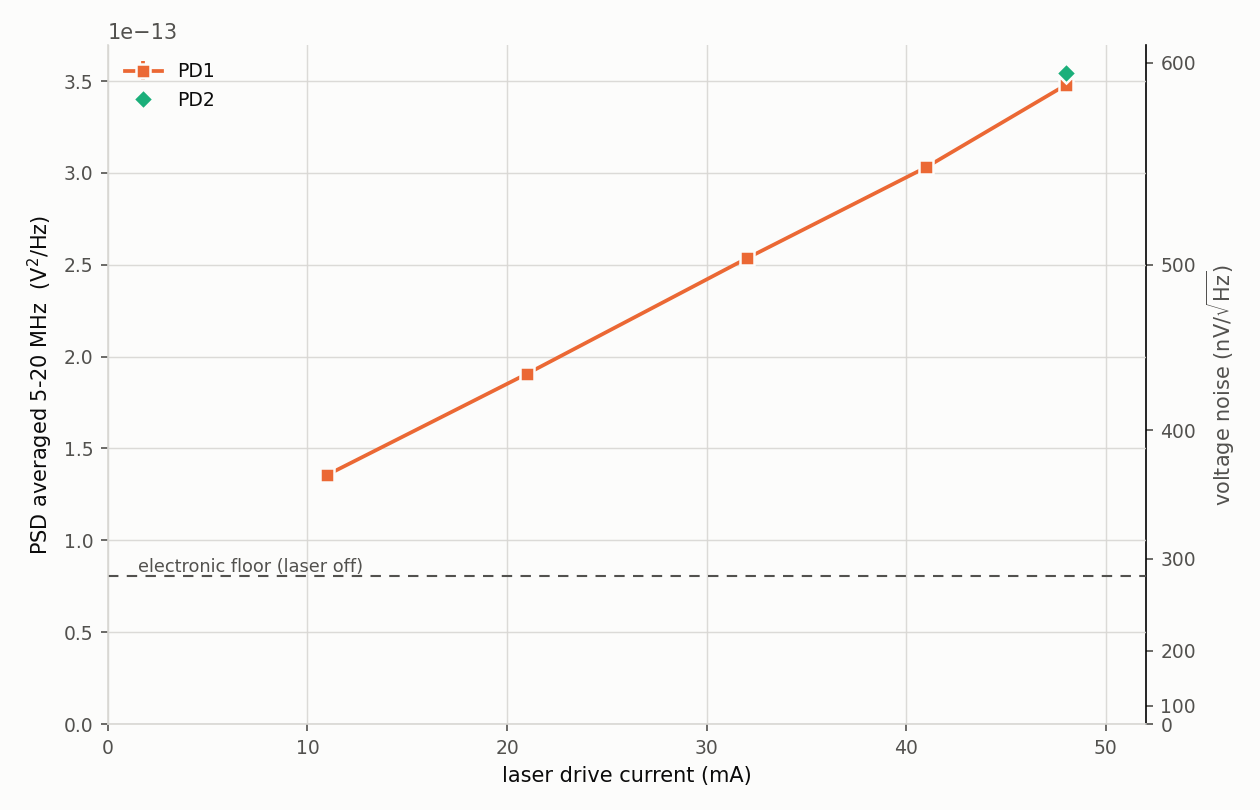
\includegraphics[width=1\linewidth]{psd_vs_current_single.png}
	\caption{A3: 5 - 20MHz Average PSD vs Laser Current with Single-Ended Detection}
	\label{fig:A3Plot}
\end{figure}

It can be seen in \autoref{fig:A3Plot} that indeed, the total noise is lower than in \autoref{fig:A2PSDvsCurrent}, as expected. Observing the total noise at the operating point of 48mA however, it can be seen that a value of approximately $3.5 \times 10^{-13}V^2/Hz$ is obtained, which gives $2.694\times 10^{-13}V^2/Hz$ once electronic noise has been subtracted. In the balanced detection case at the same laser current, a value of $5.49\times10^{-13}V^2/Hz$ was obtained - subtracting electronic noise and halving this gives $2.342\times 10^{-13}V^2/Hz$. This clearly indicates that the noise power in the single-ended case is higher than simply half of the shot-noise in the balanced detection case, thus proving that indeed there is excess RIN present. This excess RIN noise can be calculated:
\begin{equation}
	RIN_{excess}= (2.694 - 2.342)\times 10^{-13} = 0.352\times 10 ^{-13}V^2/Hz
\end{equation}

Converting to dB:

\begin{equation}
	10log_{10}(1+\frac{RIN_{excess}}{S})=10log_{10}(1+\frac{0.352\times 10 ^{-13}}{2.324\times 10^{-13}})= 0.6125dB
\end{equation}

Thus, RIN contributes an additional 0.6125dB of noise above the ideal shot-noise limit at the 48mA operating point. Balanced detection allows this excess noise to be removed, as illustrated in the results of A2 - allowing for a better SNR.
      % F  first ref: Sec 4.2.1
\chapter{Supplementary Results: Experiment D}
\label{appendix:FullWTResults}
% Referenced from: Sec 5.2.3 ("See Appendix ... for the raw PSDs of each case
% plotted on their own axes, and full tables of raw results"), and the captions
% of Tables 5.2 and 5.3 ("Full raw statistics are given in ...").

\section{Raw PSDs per Wind-tunnel Setpoint}
\label{appendix:WTPSDs}
\begin{figure}[H]
	\centering
	\includegraphics[width=0.7\linewidth]{"../Data Acquisition/figures/psd_windtunnel_cases"}
	\caption{Grid of PSD plots for each wind-tunnel setpoint}
	\label{fig:psdwindtunnelcases}
\end{figure}

\section{Raw Noise and Peak Statistics}
\label{appendix:WTRawStats}
% >>> generated: WTRawStats -- written by "Data Acquisition/make_appendixG_tables.py"; edits between these markers are overwritten
\autoref{tab:WTRawStats-fog} and \autoref{tab:WTRawStats-mist} give the un-normalised counterparts of \autoref{tab:D_snr} and \autoref{tab:D_mist_avg}: the same Doppler peaks and noise bands, but with the statistics taken on the raw PSD rather than on the PSD divided by its running-median floor. Because the raw floor slopes across the noise band, its standard deviation here includes that slope as well as the random fluctuation, which makes the raw mean $+\,5\sigma$ threshold the more conservative of the two.

\begin{table}[H]
	\centering
	\small
	\begin{tabular}{@{}S[table-format=2.1] S[table-format=2.3] S[table-format=1.2] S[table-format=1.3] S[table-format=1.2] S[table-format=1.2] S[table-format=1.2] S[table-format=2.2]@{}}
		\toprule
		{Setpoint} & {$f_D$} & \multicolumn{4}{c}{PSD ($10^{-12}$\,V$^2$/Hz)} & {Peak/mean} & {Excess} \\
		\cmidrule(lr){3-6}
		{(m/s)} & {(MHz)} & {floor mean} & {floor $\sigma$} & {mean $+\,5\sigma$} & {at $f_D$} & {(dB)} & {($10^{-7}$\,V$^2$)} \\
		\midrule
		3.1 & 3.637 & 3.01 & 0.078 & 3.41 & 4.73 & 1.96 & 10.25 \\
		5.0 & 5.868 & 3.45 & 0.075 & 3.82 & 4.79 & 1.43 & 8.87 \\
		6.0 & 6.892 & 2.44 & 0.031 & 2.59 & 3.78 & 1.90 & 7.55 \\
		7.0 & 7.997 & 2.30 & 0.040 & 2.50 & 3.49 & 1.82 & 7.04 \\
		8.0 & 9.280 & 4.30 & 0.082 & 4.71 & 5.36 & 0.95 & 5.99 \\
		9.0 & 10.611 & 2.74 & 0.042 & 2.95 & 3.60 & 1.19 & 6.08 \\
		10.0 & 11.664 & 4.20 & 0.054 & 4.46 & 5.18 & 0.92 & 6.00 \\
		11.8 & 13.837 & 3.94 & 0.053 & 4.20 & 4.51 & 0.59 & 5.27 \\
		21.0 & 24.674 & 3.69 & 0.052 & 3.95 & 4.22 & 0.59 & 4.01 \\
		\bottomrule
	\end{tabular}
	\caption{D: raw (un-normalised) noise and Doppler-peak statistics for dense fog-seeded air}
	\label{tab:WTRawStats-fog}
\end{table}

\begin{table}[H]
	\centering
	\small
	\setlength{\tabcolsep}{4.5pt}
	\begin{tabular}{@{}S[table-format=1.1] S[table-format=1.0] S[table-format=2.3] S[table-format=1.2] S[table-format=1.3] S[table-format=1.2] S[table-format=1.2] S[table-format=1.2] S[table-format=2.2]@{}}
		\toprule
		{Setpoint} & {Captures} & {$f_D$} & \multicolumn{4}{c}{PSD ($10^{-12}$\,V$^2$/Hz)} & {Peak/mean} & {Excess} \\
		\cmidrule(lr){4-7}
		{(m/s)} & {averaged} & {(MHz)} & {floor mean} & {floor $\sigma$} & {mean $+\,5\sigma$} & {at $f_D$} & {(dB)} & {($10^{-7}$\,V$^2$)} \\
		\midrule
		5.0 & 1 & 5.730 & 4.48 & 0.090 & 4.93 & {4.80\textsuperscript{\dag}} & 0.30 & 4.38 \\
		5.0 & 2 & 5.716 & 3.83 & 0.087 & 4.27 & {4.08\textsuperscript{\dag}} & 0.28 & 4.45 \\
		5.0 & 3 & 5.726 & 4.00 & 0.081 & 4.41 & {4.29\textsuperscript{\dag}} & 0.30 & 3.75 \\
		\bottomrule
	\end{tabular}

	\vspace{2pt}
	{\raggedright\footnotesize \textsuperscript{\dag}\,PSD at $f_D$ below the raw mean $+\,5\sigma$ threshold. The detection verdicts in \autoref{tab:D_mist_avg} use the floor-normalised PSD instead, on which the \SI{5}{m/s} peak clears its threshold with three captures.\par}
	\caption{D: raw (un-normalised) noise and Doppler-peak statistics for light mist-seeded air.}
	\label{tab:WTRawStats-mist}
\end{table}


\section{Velocity Accuracy: Peak Centroid vs Setpoint}
\label{appendix:velocityTable}

\autoref{tab:WTVelocity} gives the data behind \autoref{fig:figvelocityboth}: for each setpoint, the Doppler-peak centroid, the line-of-sight velocity it implies, the velocity expected from the setpoint and the \SI{35}{\degree} beam angle, and the error between the two.

\begin{table}[H]
	\centering
	\small
	\begin{tabular}{@{}S[table-format=2.1] S[table-format=2.3] S[table-format=2.2] S[table-format=2.2] S[table-format=+2.1, retain-explicit-plus]@{}}
		\toprule
		{Setpoint $U$} & {$f_D$} & {Measured $v_{\mathrm{LOS}}$} & {Expected $v_{\mathrm{LOS}}$} & {Error} \\
		{(m/s)} & {(MHz)} & {$= f_D\lambda/2$ (m/s)} & {$= U\cos 35^\circ$ (m/s)} & {(\%)} \\
		\midrule
		\multicolumn{5}{@{}l}{\textit{Collimator facing downstream (original rig)}} \\
		3.1 & 3.637 & 2.82 & 2.54 & +11.0 \\
		5.0 & 5.868 & 4.55 & 4.10 & +11.0 \\
		6.0 & 6.892 & 5.34 & 4.91 & +8.7 \\
		7.0 & 7.997 & 6.20 & 5.73 & +8.1 \\
		8.0 & 9.280 & 7.19 & 6.55 & +9.8 \\
		9.0 & 10.611 & 8.22 & 7.37 & +11.6 \\
		10.0 & 11.664 & 9.04 & 8.19 & +10.4 \\
		11.8 & 13.837 & 10.72 & 9.67 & +10.9 \\
		21.0 & 24.674 & 19.12 & 17.20 & +11.2 \\
		\multicolumn{5}{@{}l}{\quad Fit through origin: \SI{1.170 \pm 0.003}{MHz} per m/s, +10.7\,\% above the expected \SI{1.057}{MHz} per m/s} \\
		\midrule
		\multicolumn{5}{@{}l}{\textit{Collimator facing upstream (rotated rig)}} \\
		3.9 & 4.269 & 3.31 & 3.19 & +3.6 \\
		5.3 & 5.733 & 4.44 & 4.34 & +2.3 \\
		6.1 & 6.802 & 5.27 & 5.00 & +5.5 \\
		6.3 & 6.816 & 5.28 & 5.16 & +2.4 \\
		7.5 & 8.422 & 6.53 & 6.14 & +6.2 \\
		8.0 & 9.105 & 7.06 & 6.55 & +7.7 \\
		9.0 & 10.265 & 7.95 & 7.37 & +7.9 \\
		10.0 & 11.337 & 8.79 & 8.19 & +7.3 \\
		21.0 & 23.864 & 18.49 & 17.20 & +7.5 \\
		\multicolumn{5}{@{}l}{\quad Fit through origin: \SI{1.130 \pm 0.006}{MHz} per m/s, +6.9\,\% above the expected \SI{1.057}{MHz} per m/s} \\
		\bottomrule
	\end{tabular}
	
	\caption{D: Doppler-peak centroid and line-of-sight velocity against the wind-tunnel setpoint for both rig orientations, in dense fog-seeded air}
	\label{tab:WTVelocity}
\end{table}

      % G  first ref: Sec 5.2.3
\chapter{Use of AI Tools}
\label{appendix:AIUse}
% Template requirement: "If you have used AI in writing your report, you need
% to provide details in one of the appendices of how you used it."
% TODO: describe which tools were used and for what (e.g. editing for length
% and clarity, LaTeX/TikZ formatting of figures and tables, checking
% calculations, CAD scripts for the test rigs), and state that all design
% decisions, experiments, data and conclusions are your own.
                % H  template-mandated
\chapter{Code and Additional Materials}
\label{appendix:code}
% Template requirement (optional): link to a GitHub repository with the code
% and additional materials.
% TODO: add the repository URL and a one-paragraph description of its contents
% (oscilloscope acquisition scripts, Welch PSD / peak-detection processing,
% plotting scripts, raw data, and the OpenSCAD files for the hard-target rig,
% wind-tunnel wedge and enclosure).
                  % I  template-mandated
\chapter{Ethics Forms}
\label{appendix:ethics}

\begin{figure}[H]
	\centering
	\includegraphics[width=0.85\linewidth]{"../../../../../Downloads/report (1)"}
	\caption{}
	\label{fig:report-1}
\end{figure}
                % J  Addenda
